\chapter{System Diagrams}

\begin{figure}[H]
	\centering
	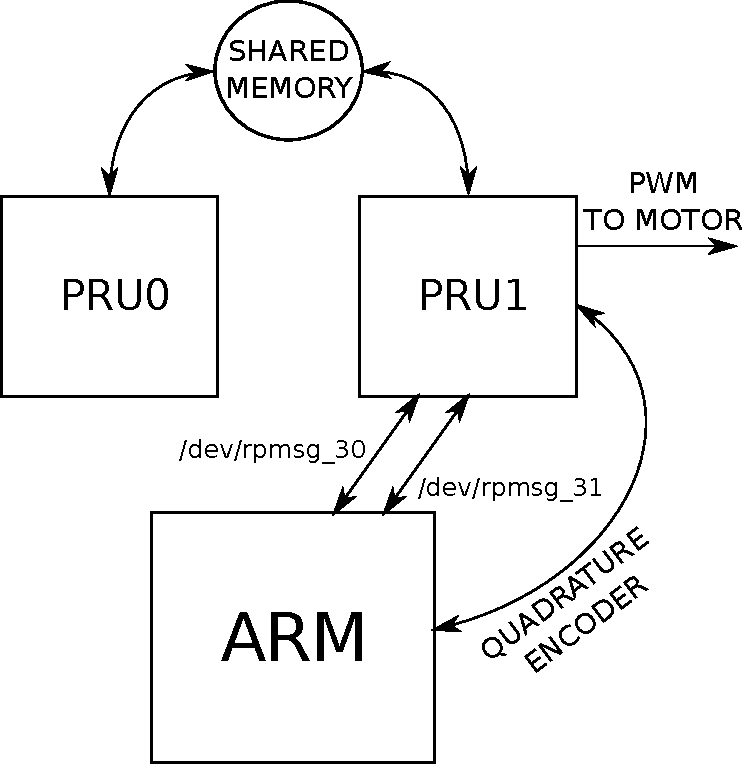
\includegraphics[width=0.8\textwidth]{diagrams/soc_system}
	\centering\bfseries
	\caption{PRU PID System on BeagleBone Green AM335X ``System On Chip''}
\end{figure}

The above diagram shows the data pathways used in the project.

\section{Programmable Real-time Units (PRU)}

The system uses both PRUs available on the Beaglebone Green:

\begin{enumerate}
\item 

PRU0 implements the PID controller.  The C code in file PRU\_PID\_0.c contains
the math required for the PID controller.  The controlled quantity is the DC motor RPM which is obtained from the Quadrature Encoder.

PRU0 gets performs calculations based on data retrieved (and written to) PRU shared memory.
\item 
PRU1 acts as the master communicator for the system.  PRU1 instantiates two "character devices" via the RemoteProc Messaging framework.  These character devices are used for two-way communication between the PRUs and Linux user-space.  In addition to the supervisory control function, the PWM module on PRU1 is used to drive the DC motor driver IC.

The Quadrature encoder used is not part of the PRU-ICSS.  However, the PRUs have access to the encoders which are part of the AM335X "System On Chip" (SOC).  Access to this encoder is enabled in PRU1 code.
\end{enumerate}

It is worth noting that the PRUs each have a copy of the same ``PWMSS'' (Pulse-Width Modulation Subsystem) as the ones located in the AM335X SOC.  However, only a single pin is connected from the PRU-ICSS to the outside world.  Since this single pin is used for PWM, the decoder-counter function must be done outside the PRU-ICSS thus one of the SOC's eQEP decoder-counters is used and is accessed by PRU1 via the Interface/OCP Master port.

The PWMSS sub-system is surprisingly complex.  A detailed description of the features of this sub-system is available in the AM335x Technical Reference Manual:

\url{http://www.ti.com/lit/ug/spruh73o/spruh73o.pdf}

\section{PRU Shared Memory}

The firmwares running on the two PRUs use a C structure which is placed into "shared memory".  The shared memory is a feature built into the PRU-ICSS architecture.  The shared memory is allocated by an entry in the "linker command file" which is included in the Github repository.

The structure in shared memory allows the two PRUs to synchronize the PID control parameters.  PRU1 receives the parameters via user-space via the character devices and then writes them to shared memory.  This makes the parameters available to PRU0, which is then able to perform PID control loop calculations.  In turn, PRU0 calculates the PWM duty cycle, and this is written to shared memory.  PRU1 then applies this to the PWM output.

PRU1 is responsible for reading the Quadrature Encoder, which is accessed via the OCP bus master.  PRU1 writes this data to shared memory, which enables PRU0 to access this information for PID loop calculations.

A mystery is how the PRUs are able to share memory without locking.  It is possible for the PRUs to simultaneously read and write to the same memory location without introducing errors?

